\section{Permutations and combinations}

\begin{theorem*}
  The number of $k$-tuples that can be formed from $\{1, 2, \ldots, n\}$ is
  \begin{align*}
    P(n, k) = n_{(k)} = n(n-1)(n-2)\cdots(n-k+1).
  \end{align*}
  The number of sets of size $k$ that can be formed from $\{1, 2, \ldots, n\}$ is
  \begin{align*}
    C(n, k) = {n \choose k} = \frac{P(n, k)}{k!}.
  \end{align*}
\end{theorem*}

\section{Binomial theorem}
\begin{align*}
  (a + b)^n = \sum_{k=0}^n{n \choose k}a^{n-k}b^k
\end{align*}

\section{Triangle inequalities}

\begin{theorem*}
  Let $a, b \in \R$ with $a \neq b$ and $a, b \neq 0$. Using $+$, $-$ and $|\cdot|$ we can generate the
  following 4 real numbers:
  \begin{align*}
    -\big(|a| + |b|\big) ~~~ < ~~~
    -\big||a| - |b|\big| ~~~ < ~~~
    0                    ~~~ < ~~~
    \big||a| - |b|\big|  ~~~ < ~~~
    |a| + |b|.
  \end{align*}
  \begin{itemize}
  \item $a + b$ and $a - b$ can equal any of them.
  \item $|a + b|$ and $|a - b|$ can equal either of the two positive numbers.
  \item $|a| - |b|$ can equal either of the two ``inner'' numbers.
  \end{itemize}
  ~\\~\\
  If we allow $a = b$ with $ a \neq 0, b \neq 0$ then
  \begin{align*}
    -\big(|a| + |b|\big) ~~~ < ~~~
    -\big||a| - |b|\big| ~~~ \red{\leq} ~~~
    0                    ~~~ \red{\leq} ~~~
    \big||a| - |b|\big|  ~~~ < ~~~
    |a| + |b|.
  \end{align*}
  If we allow $a = 0$ and $b = 0$ with $a \neq b$ then
  \begin{align*}
    -\big(|a| + |b|\big) ~~~ \red{\leq} ~~~
    -\big||a| - |b|\big| ~~~ < ~~~
    0                    ~~~ < ~~~
    \big||a| - |b|\big|  ~~~ \red{\leq} ~~~
    |a| + |b|;
  \end{align*}
  If we allow $a = b$ including $a = b = 0$ then
  \begin{align*}
    -\big(|a| + |b|\big) ~~~ \red{\leq} ~~~
    -\big||a| - |b|\big| ~~~ \red{\leq} ~~~
    0                    ~~~ \red{\leq} ~~~
    \big||a| - |b|\big|  ~~~ \red{\leq} ~~~
    |a| + |b|;
  \end{align*}
\end{theorem*}

\section{The quadratic formula}

\begin{theorem*}
  The roots of $ax^2 + bx + c = 0$ are $x = \frac{-b \pm \sqrt{b^2 - 4ac}}{2a}$.
\end{theorem*}

\begin{proof}
  \begin{align*}
    x^2 + \frac{b}{a}x + \frac{c}{a}                        &= 0\\
    \(x + \frac{b}{2a}\)^2 - \frac{b^2}{4a^2} + \frac{c}{a} &= 0 ~~~~~~~~~~~~~~~~~~~~~\text{``completing the square"}\\
    x &= -\frac{b}{2a} \pm \sqrt{\frac{b^2}{4a^2} - \frac{4ac}{4a^2}}\\
                                                            &= \frac{-b \pm \sqrt{b^2 - 4ac}}{2a}.
  \end{align*}
\end{proof}

\section{Geometric series}
\begin{theorem*}
  $a_n := \sum_{k=0}^nr^k = \frac{~~~~1 - r^{n+1}}{1 - r}$.

  Therefore if $r < 1$ then $\lim_{n \to \infty} a_n = \frac{1}{1 - r}$.
\end{theorem*}
\begin{proof}
  \begin{align*}
    a_n          &= \sum_{k=0}^nr^n = 1 + r + r^2 + \ldots + r^n\\
    a_n - ra_n  &= 1 - r^{n+1}\\
    a_n          &= \frac{~~~~1 - r^{n+1}}{1 - r}
  \end{align*}
\end{proof}
\begin{remark*}
  Note that $a_{n+1} = 1 + ra_n$.
\end{remark*}

\section{Partial fractions}

\red{TODO}

\section{Even and odd functions}

\begin{definition*}
  A function (over an additive group?) is even if $f(-x) = f(x)$ for all $x$.

  A function (over an additive group?) is odd if $f(-x) = -f(x)$ for all $x$.
\end{definition*}

Functions can be neither even nor odd.

\begin{claim*}
  A polynomial $p(x)$ is even if an only if it has only even powers of $x$.

  A polynomial $p(x)$ is odd if an only if it has only odd powers of $x$.
\end{claim*}

\section{Convex and concave functions}\label{convexity}
A real-valued function $f:\R\to\R$ is \defn{convex} over an interval $[x_1, x_2]$ if the line
segment joining $f(x_1)$ to $f(x_2)$ lies above the graph of $f$, i.e. if
\begin{align*}
  pf(x_1) + (1-p)f(x_2) \geq f(px_1 + (1 - p)x_2).
\end{align*}
E.g. $x \mapsto x^2$ and $x \mapsto e^x$ are convex.

A real-valued function $f$ is \defn{concave} if $-f$ is convex. These definitions extend to
real-valued functions $f$ over an $n$-dimensional interval / convex set\footnote{ Basically, a set
  which includes all points on line segments joining points in the set.}.

\section{Trigonometric identities}
\begin{align*}
  \cos 2\theta &= \cos^2\theta - \sin^2\theta
\end{align*}

\section{Hyperbolic trigonometric functions}\label{foundations-hyperbolic-trig-functions}

Define
\begin{align*}
  \cosh x &= \frac{e^x + e^{-x}}{2} \\
  \sinh x &= \frac{e^x - e^{-x}}{2}.
\end{align*}
Therefore
\begin{align*}
  \ddx \cosh x &= \sinh x \\
  \ddx \sinh x &= \cosh x,
\end{align*}
and
\begin{align*}
  \cosh^2 x             &= \frac{1}{4}\(e^{2x} + e^{-2x}\) + \frac{1}{2} \\
  \sinh^2 x             &= \frac{1}{4}\(e^{2x} + e^{-2x}\) - \frac{1}{2} \\
  1 + \sinh^2 x         &= \cosh^2 x \\
  \sinh^2 x + \cosh^2 x &= \cosh 2x
\end{align*}

$\sin$ and $\sinh$ are odd, and $\cos$ and $\cosh$ are even.

Note that these functions equal their own second derivatives. I.e. they provide solutions to
\begin{align*}
  \ddot{x} - x = 0.
\end{align*}
In contrast, $\sin$ and $\cos$ equal the negative of their own second derivative, so they provide
solutions to
\begin{align*}
  \ddot{x} + x = 0.
\end{align*}

\subsection*{\url{https://www.reddit.com/r/explainlikeimfive/comments/61siyw/eli5_can_someone_explain_the_hyperbolic_trig/}}

They are a bit mysterious, but not at all scary. It is just a way of grouping the exponential
functions into even and odd components.

From calculus, you know the relationship between the exponential and the standard trig functions:

\begin{align*}
e^{ix} = cos x + i sin x
\end{align*}

That works for imaginary arguments to the exponential and it splits it into a real and even
component (cosine) and an imaginary and odd component (sine). That is the solution to this
differential equation

\begin{align*}
  \ddot{y} + y = 0.
\end{align*}

Those functions are equal to the opposite sign of the second
derivative.

What about this differential equation:

\begin{align*}
  \ddot{y} - y = 0
\end{align*}

where the function is equal to its second derivative? Those solutions are simply $e^x$ and $e^{-x}$
. But neither of those solutions are even or odd. You could re-group those two solutions so that you
have an even solution and an odd solution.

\begin{align*}
e^x + e^{-x} &= (1/2) (e^x + e^{-x} ) + (1/2) (e^x - e^{-x} )
\end{align*}
They define the even solution to be hyperbolic cosine and the odd solution to be hyperbolic sine.

\begin{align*}
e^x + e^{-x} &= cosh x + sinh x
\end{align*}
So the definitions of the regular and hyperbolic trig functions with relation to the exponentials
are:

\begin{align*}
cos x &= (1/2) ( e^{ix} + e^{-ix} ) \\
sin x &= (1/2i) ( e^{ix} - e^{-ix} )
\end{align*}
and

\begin{align*}
cosh x &= (1/2) ( e^x + e^{-x} ) \\
sinh x &= (1/2) ( e^x - e^{-x} )
\end{align*}

You can see the analogy! From there, they can work out more algebra and calculus to see if there's
any other useful relations that make this splitting of the expontial into even and odd components
helpful. But it is not as crucial that you work with the hyperbolic functions this way. You could
choose to leave the solutions in their $e^{x}$ and $e^{-x}$ . Many times it helps, but its use is
not as common as the standard trig functions.



\section{$\sqrt{2}$ is irrational}
\begin{theorem*}
  $\sqrt{2}$ is irrational.
\end{theorem*}

\begin{proof}
  Suppose $\sqrt{2} \in \Q$. Then $\sqrt{2}$ can be written as $\frac{a}{b}$ where $a, b \in \Z$
  have no common factor (aka coprime, aka mutually prime).

  Then $2 = \frac{a^2}{b^2}$, so $a^2$ is even.

  Therefore $a$ is even.

  Let $a = 2c$. Then $b^2 = \frac{4c^2}{2} = 2c^2$, so $b^2$ is even.

  Therefeore both $a$ and $b$ are even, which is a contradiction.

  Therefore $\sqrt{2} \notin \Q$.
\end{proof}

\begin{remark*}
  It remains to be proved that $\sqrt{2}$ exists in $\R$. See \ref{existence-of-root-2}.
\end{remark*}

\section{Misc}
\begin{mdframed}
  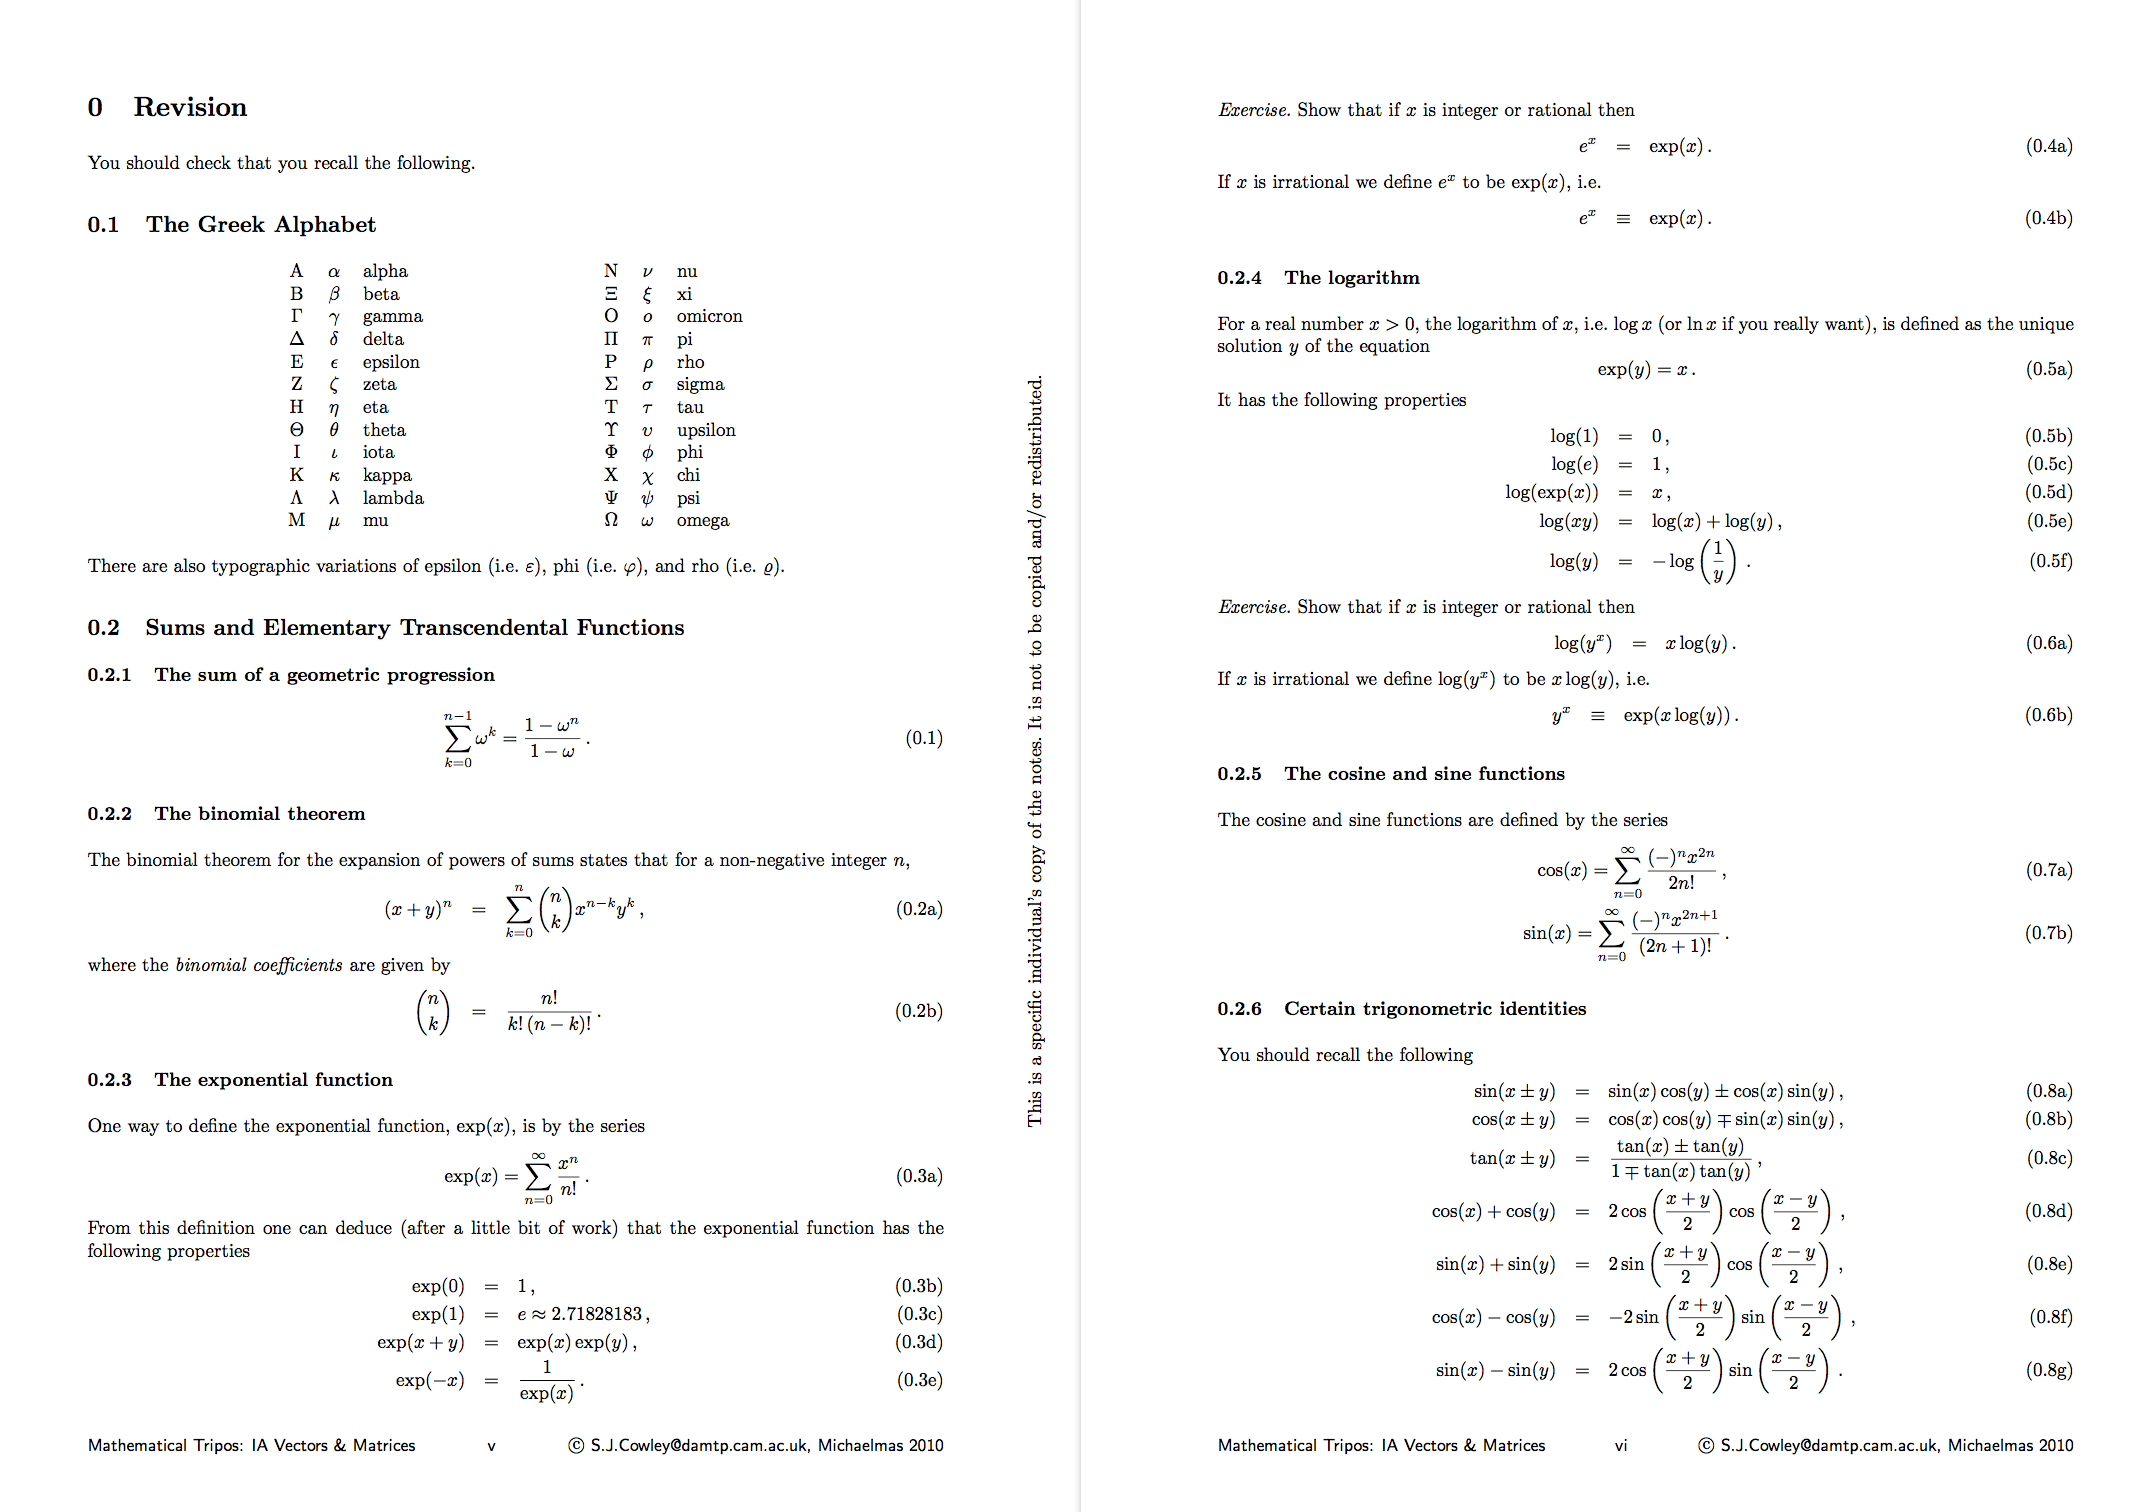
\includegraphics[width=400pt]{img/misc--cambridge-1a-vectors-and-matrices-revision-1.png}
\end{mdframed}
\begin{mdframed}
  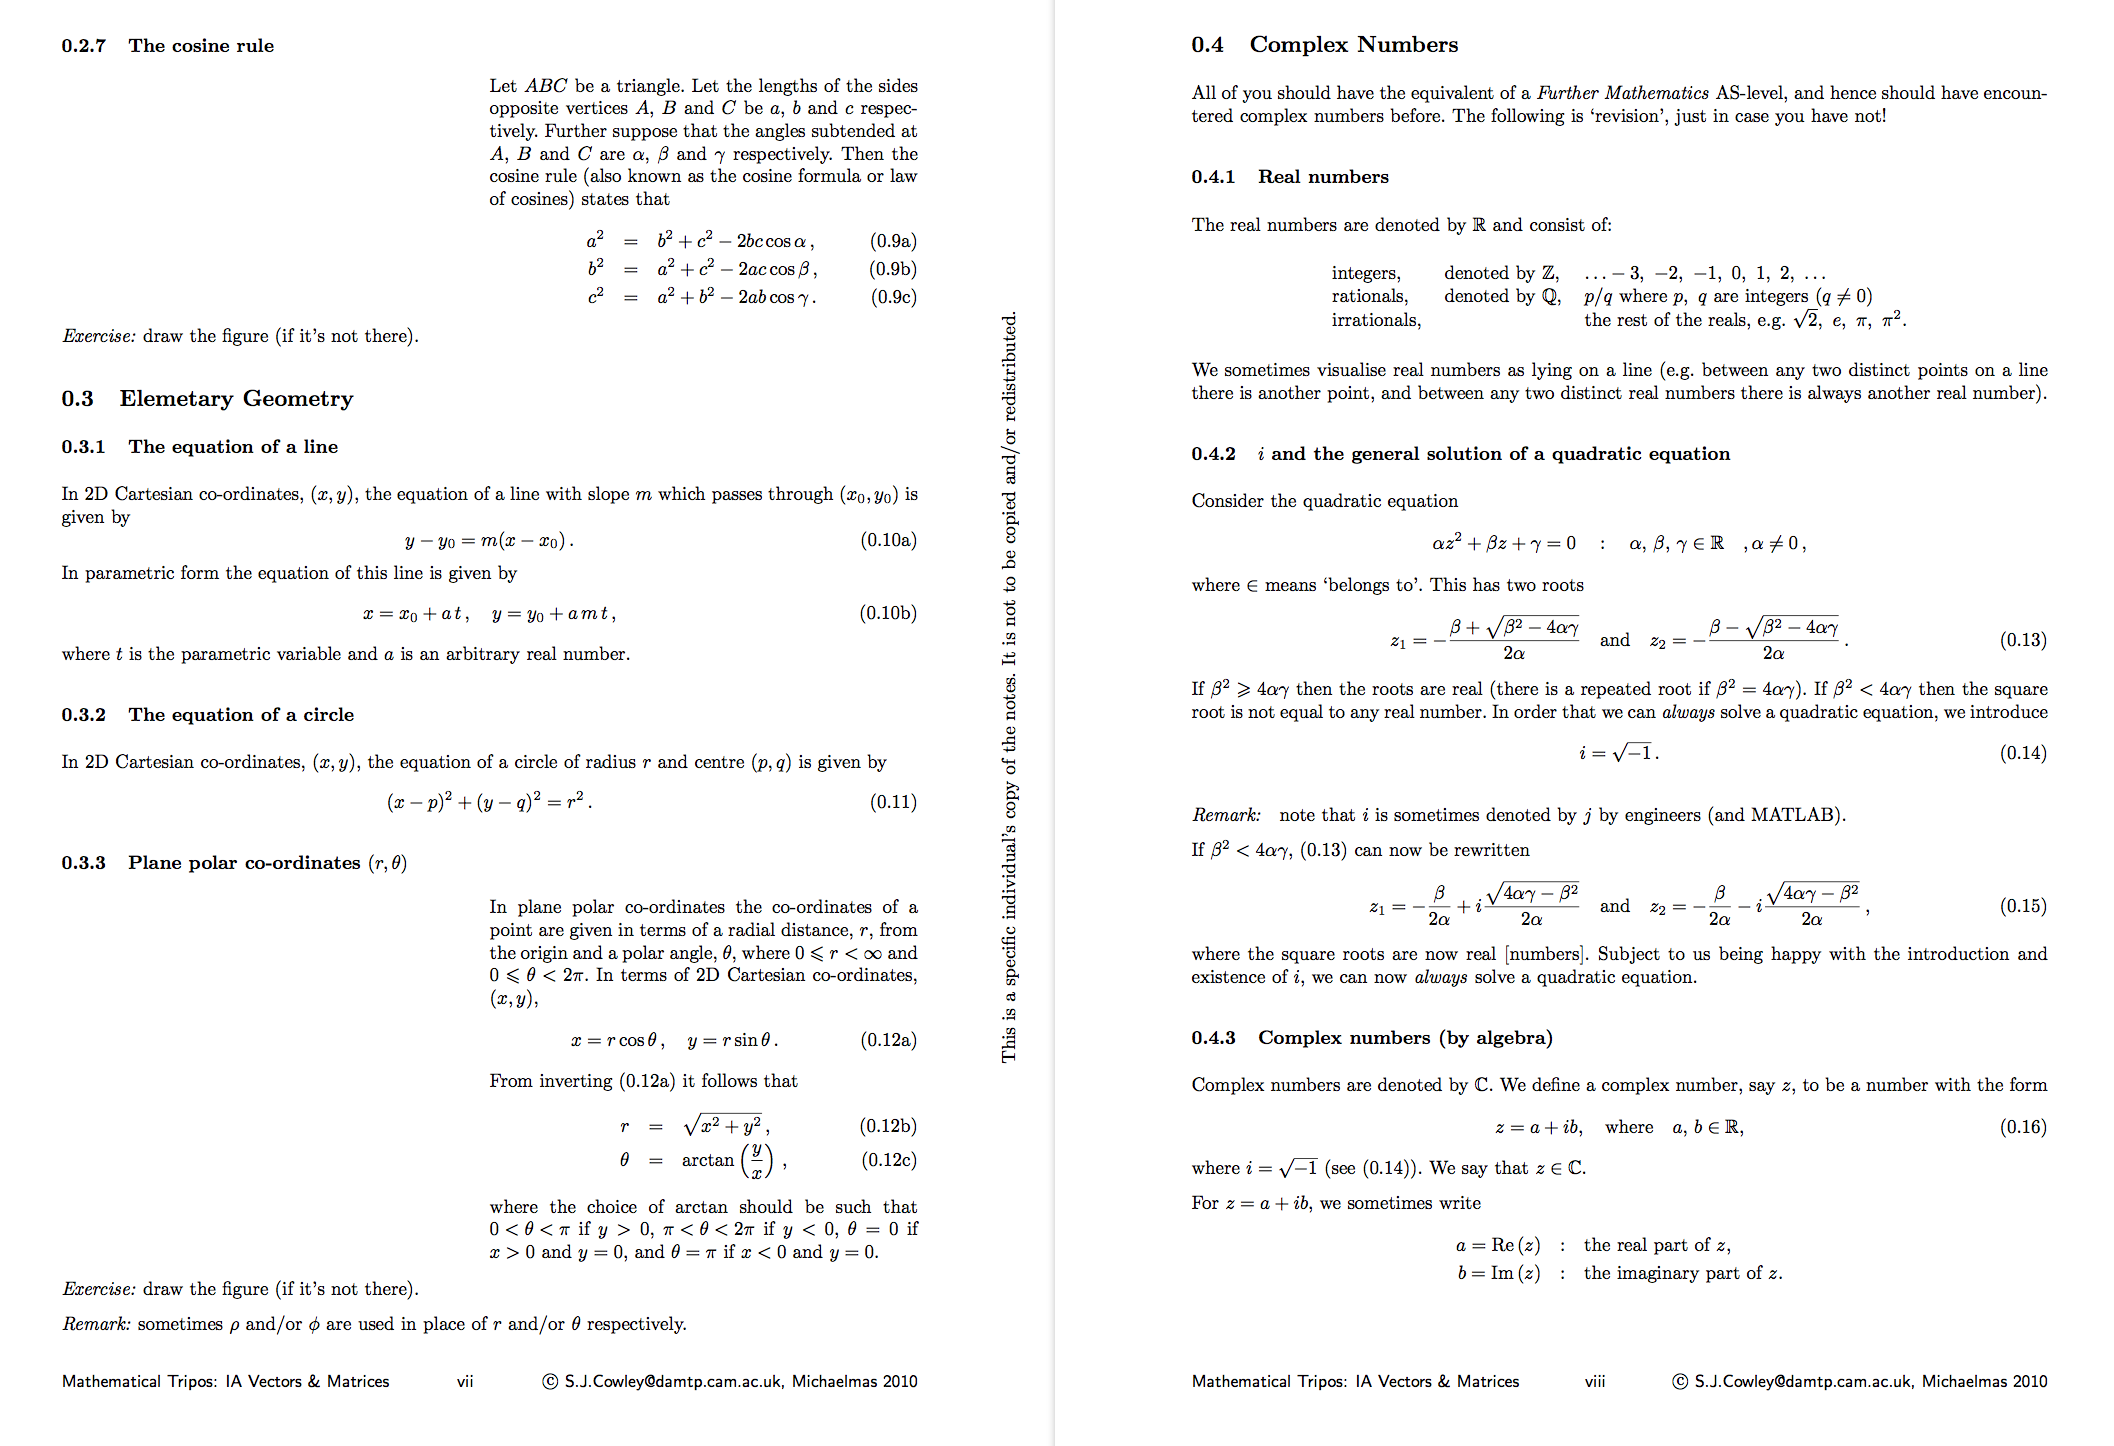
\includegraphics[width=400pt]{img/misc--cambridge-1a-vectors-and-matrices-revision-2.png}
\end{mdframed}
\begin{mdframed}
  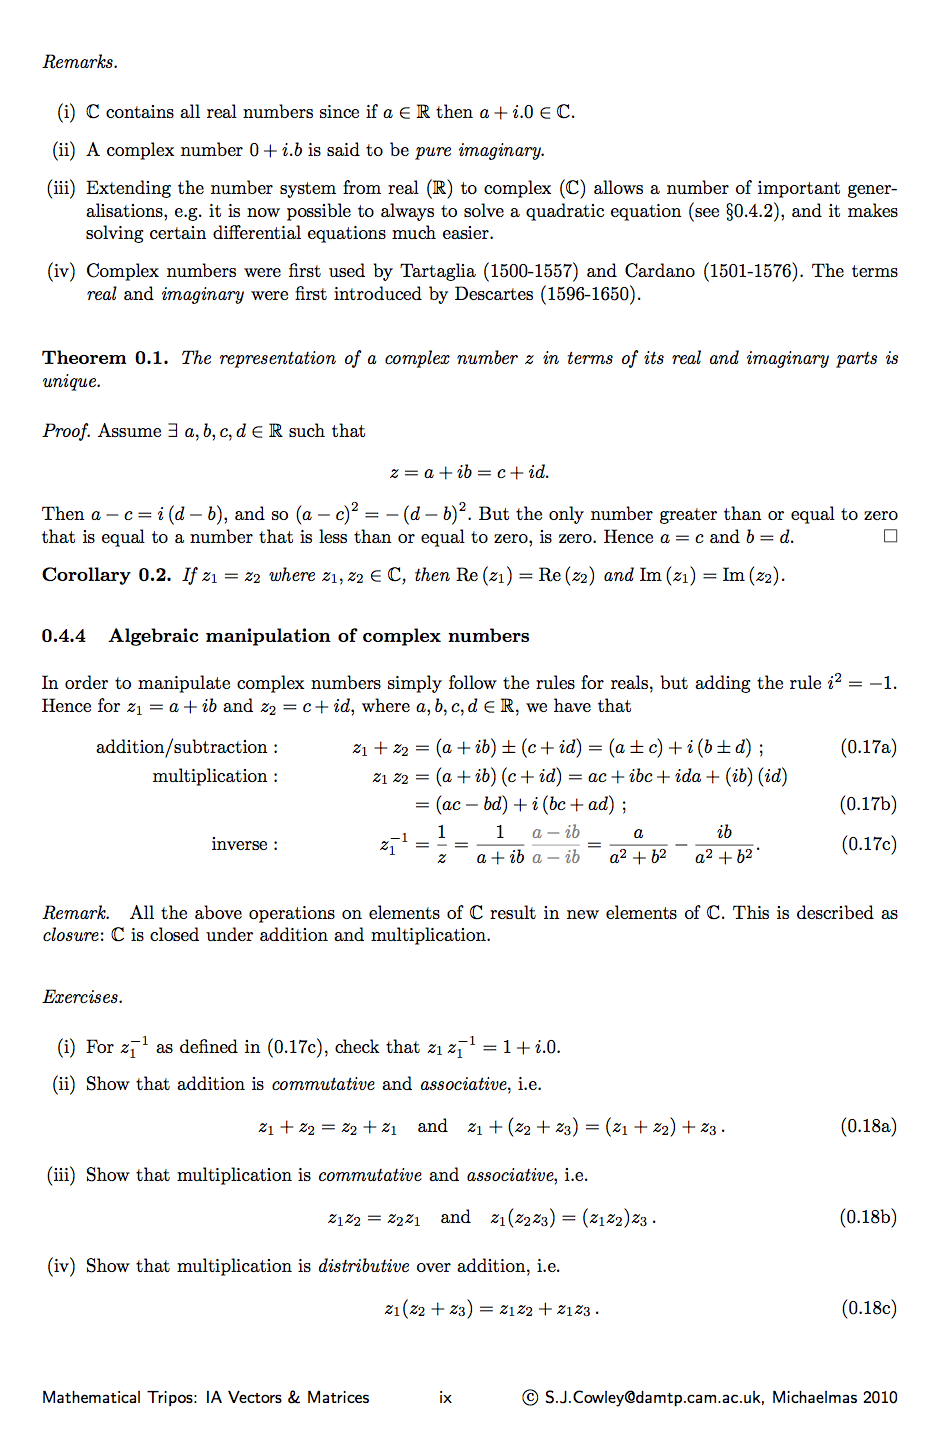
\includegraphics[width=400pt]{img/misc--cambridge-1a-vectors-and-matrices-revision-3.png}
\end{mdframed}


\begin{claim*}
  The sum of the first $n$ odd numbers equals $n^2$.
\end{claim*}

The claim is that $ = n^2$.

Note that by drawing patterns of dots we see that $\sum_{i=1}^n i$ can always be arranged to form
the upper triangle of a square, including the diagonal. Therefore
$\sum_{i=1}^n i = \frac{n^2 - n}{2} + n = \frac{n(n+1)}{2}$, and

\begin{align*}
  \sum_{i=1}^n (2i - 1)
  &= 2\sum_{i=1}^n i - n \\
  &= 2\frac{n(n+1)}{2} - n \\
  &= n^2.
\end{align*}
